% Options for packages loaded elsewhere
\PassOptionsToPackage{unicode}{hyperref}
\PassOptionsToPackage{hyphens}{url}
%
\documentclass[
]{article}
\usepackage{amsmath,amssymb}
\usepackage{iftex}
\ifPDFTeX
  \usepackage[T1]{fontenc}
  \usepackage[utf8]{inputenc}
  \usepackage{textcomp} % provide euro and other symbols
\else % if luatex or xetex
  \usepackage{unicode-math} % this also loads fontspec
  \defaultfontfeatures{Scale=MatchLowercase}
  \defaultfontfeatures[\rmfamily]{Ligatures=TeX,Scale=1}
\fi
\usepackage{lmodern}
\ifPDFTeX\else
  % xetex/luatex font selection
\fi
% Use upquote if available, for straight quotes in verbatim environments
\IfFileExists{upquote.sty}{\usepackage{upquote}}{}
\IfFileExists{microtype.sty}{% use microtype if available
  \usepackage[]{microtype}
  \UseMicrotypeSet[protrusion]{basicmath} % disable protrusion for tt fonts
}{}
\makeatletter
\@ifundefined{KOMAClassName}{% if non-KOMA class
  \IfFileExists{parskip.sty}{%
    \usepackage{parskip}
  }{% else
    \setlength{\parindent}{0pt}
    \setlength{\parskip}{6pt plus 2pt minus 1pt}}
}{% if KOMA class
  \KOMAoptions{parskip=half}}
\makeatother
\usepackage{xcolor}
\usepackage[margin=1in]{geometry}
\usepackage{color}
\usepackage{fancyvrb}
\newcommand{\VerbBar}{|}
\newcommand{\VERB}{\Verb[commandchars=\\\{\}]}
\DefineVerbatimEnvironment{Highlighting}{Verbatim}{commandchars=\\\{\}}
% Add ',fontsize=\small' for more characters per line
\usepackage{framed}
\definecolor{shadecolor}{RGB}{248,248,248}
\newenvironment{Shaded}{\begin{snugshade}}{\end{snugshade}}
\newcommand{\AlertTok}[1]{\textcolor[rgb]{0.94,0.16,0.16}{#1}}
\newcommand{\AnnotationTok}[1]{\textcolor[rgb]{0.56,0.35,0.01}{\textbf{\textit{#1}}}}
\newcommand{\AttributeTok}[1]{\textcolor[rgb]{0.13,0.29,0.53}{#1}}
\newcommand{\BaseNTok}[1]{\textcolor[rgb]{0.00,0.00,0.81}{#1}}
\newcommand{\BuiltInTok}[1]{#1}
\newcommand{\CharTok}[1]{\textcolor[rgb]{0.31,0.60,0.02}{#1}}
\newcommand{\CommentTok}[1]{\textcolor[rgb]{0.56,0.35,0.01}{\textit{#1}}}
\newcommand{\CommentVarTok}[1]{\textcolor[rgb]{0.56,0.35,0.01}{\textbf{\textit{#1}}}}
\newcommand{\ConstantTok}[1]{\textcolor[rgb]{0.56,0.35,0.01}{#1}}
\newcommand{\ControlFlowTok}[1]{\textcolor[rgb]{0.13,0.29,0.53}{\textbf{#1}}}
\newcommand{\DataTypeTok}[1]{\textcolor[rgb]{0.13,0.29,0.53}{#1}}
\newcommand{\DecValTok}[1]{\textcolor[rgb]{0.00,0.00,0.81}{#1}}
\newcommand{\DocumentationTok}[1]{\textcolor[rgb]{0.56,0.35,0.01}{\textbf{\textit{#1}}}}
\newcommand{\ErrorTok}[1]{\textcolor[rgb]{0.64,0.00,0.00}{\textbf{#1}}}
\newcommand{\ExtensionTok}[1]{#1}
\newcommand{\FloatTok}[1]{\textcolor[rgb]{0.00,0.00,0.81}{#1}}
\newcommand{\FunctionTok}[1]{\textcolor[rgb]{0.13,0.29,0.53}{\textbf{#1}}}
\newcommand{\ImportTok}[1]{#1}
\newcommand{\InformationTok}[1]{\textcolor[rgb]{0.56,0.35,0.01}{\textbf{\textit{#1}}}}
\newcommand{\KeywordTok}[1]{\textcolor[rgb]{0.13,0.29,0.53}{\textbf{#1}}}
\newcommand{\NormalTok}[1]{#1}
\newcommand{\OperatorTok}[1]{\textcolor[rgb]{0.81,0.36,0.00}{\textbf{#1}}}
\newcommand{\OtherTok}[1]{\textcolor[rgb]{0.56,0.35,0.01}{#1}}
\newcommand{\PreprocessorTok}[1]{\textcolor[rgb]{0.56,0.35,0.01}{\textit{#1}}}
\newcommand{\RegionMarkerTok}[1]{#1}
\newcommand{\SpecialCharTok}[1]{\textcolor[rgb]{0.81,0.36,0.00}{\textbf{#1}}}
\newcommand{\SpecialStringTok}[1]{\textcolor[rgb]{0.31,0.60,0.02}{#1}}
\newcommand{\StringTok}[1]{\textcolor[rgb]{0.31,0.60,0.02}{#1}}
\newcommand{\VariableTok}[1]{\textcolor[rgb]{0.00,0.00,0.00}{#1}}
\newcommand{\VerbatimStringTok}[1]{\textcolor[rgb]{0.31,0.60,0.02}{#1}}
\newcommand{\WarningTok}[1]{\textcolor[rgb]{0.56,0.35,0.01}{\textbf{\textit{#1}}}}
\usepackage{longtable,booktabs,array}
\usepackage{calc} % for calculating minipage widths
% Correct order of tables after \paragraph or \subparagraph
\usepackage{etoolbox}
\makeatletter
\patchcmd\longtable{\par}{\if@noskipsec\mbox{}\fi\par}{}{}
\makeatother
% Allow footnotes in longtable head/foot
\IfFileExists{footnotehyper.sty}{\usepackage{footnotehyper}}{\usepackage{footnote}}
\makesavenoteenv{longtable}
\usepackage{graphicx}
\makeatletter
\def\maxwidth{\ifdim\Gin@nat@width>\linewidth\linewidth\else\Gin@nat@width\fi}
\def\maxheight{\ifdim\Gin@nat@height>\textheight\textheight\else\Gin@nat@height\fi}
\makeatother
% Scale images if necessary, so that they will not overflow the page
% margins by default, and it is still possible to overwrite the defaults
% using explicit options in \includegraphics[width, height, ...]{}
\setkeys{Gin}{width=\maxwidth,height=\maxheight,keepaspectratio}
% Set default figure placement to htbp
\makeatletter
\def\fps@figure{htbp}
\makeatother
\setlength{\emergencystretch}{3em} % prevent overfull lines
\providecommand{\tightlist}{%
  \setlength{\itemsep}{0pt}\setlength{\parskip}{0pt}}
\setcounter{secnumdepth}{5}
\ifLuaTeX
  \usepackage{selnolig}  % disable illegal ligatures
\fi
\IfFileExists{bookmark.sty}{\usepackage{bookmark}}{\usepackage{hyperref}}
\IfFileExists{xurl.sty}{\usepackage{xurl}}{} % add URL line breaks if available
\urlstyle{same}
\hypersetup{
  pdftitle={Feature Selection and Extraction},
  pdfauthor={Cheng Peng},
  hidelinks,
  pdfcreator={LaTeX via pandoc}}

\title{Feature Selection and Extraction}
\author{Cheng Peng}
\date{STA 551 Foundations of Data Science}

\begin{document}
\maketitle

{
\setcounter{tocdepth}{4}
\tableofcontents
}
\hypertarget{introduction}{%
\section{Introduction}\label{introduction}}

Feature selection is a critical and widely used technique in data
processing, aimed at selecting the most relevant features from noisy
data. This approach not only enhances the execution speed of data
processing algorithms but also improves prediction accuracy and reduces
variability in results.

\hypertarget{feature-selection-methods}{%
\section{Feature Selection Methods}\label{feature-selection-methods}}

Feature selection, a dimensionality reduction technique, focuses on
identifying a small subset of relevant features from the original
dataset by eliminating irrelevant, redundant, or noisy features. This
process typically enhances learning performance, improves model
accuracy, reduces computational costs, and increases model
interpretability.

Several statistical methods relevant to feature selection have been
discussed in various statistics courses. This section provides an
overview of feature selection types, methodologies, and techniques
commonly employed in both statistics and machine learning. Based on
their nature, these methods are categorized into four distinct types,
which will be outlined in the following subsections.

\hypertarget{filter-methods}{%
\subsection{Filter Methods}\label{filter-methods}}

Filter methods are statistical-based feature selection methods that
involve evaluating the relationship between each input variable and the
target (response) variable using statistics and selecting those input
variables that have the strongest relationship with the target variable.
These methods can be fast and effective, although the choice of
statistical measures depends on the data type of both the input and
output variables. Here are some of these methods with brief
descriptions.

\hypertarget{information-gain}{%
\subsubsection{Information Gain}\label{information-gain}}

Information gain calculates the reduction in entropy from the
transformation of a data set. It can be used for feature selection by
evaluating the Information gain of each variable in the context of the
target variable. We have briefly described this method in decision
induction.

\hypertarget{chi-square-test}{%
\subsubsection{Chi-square Test}\label{chi-square-test}}

Let's consider a scenario where we need to determine the relationship
between the independent category feature (predictor) and dependent
category feature(response). In feature selection, we aim to select the
features which are highly dependent on the response. We calculate
Chi-square between each feature and the response variable. and select
the desired number of features with the best Chi-square scores.

In order to correctly apply the chi-squared test for the relationship
between various features in the data set and the target variable, the
following conditions have to be met: the variables have to be
categorical, sampled independently and values should have an expected
frequency greater than 5.

\hypertarget{fishers-score}{%
\subsubsection{Fisher's Score}\label{fishers-score}}

Fisher score is one of the most widely used supervised feature selection
methods. It seeks features with the best discriminant ability. It is
based on maximizing the distances between data points of different
classes and minimizing the distances among points of the same class. To
rank the features in the order of their relevancy, they are sorted in
the decreasing order of their obtained fisher score. Thus, as the value
of an assigned score to a feature increases, its importance also
increases.

Let \(Y\) be the categorical variable with \(C\) categories and \(X\) be
a numerical variable. The Fisher's score of \(X\) is defined by

\[
F_X = \frac{\sum_{i=1}^C N_i(\mu_{X}^i-\mu_{X})^2}{\sum_{i=1}^CN_i\times (\sigma_X^i)^2}
\] where \(N_i\) is the number of data points in class \(i\), \(\mu_X\)
is the mean of feature variable \(X\), and \(\mu_X^i\) and
\((\sigma_X^i)^2\) are the mean and the variance of class \(i\) upon the
feature \(X\) respectively.

The algorithm returns the ranks of the variables based on the fisher's
score in descending order. We can then select the variables based on the
scores.

\hypertarget{correlation-coefficient}{%
\subsubsection{Correlation Coefficient}\label{correlation-coefficient}}

Correlation is a measure of the linear relationship of 2 or more
variables. Through correlation, we can predict one variable from the
other. The logic behind using correlation for feature selection is that
the good variables are highly correlated with the response. Furthermore,
variables should be correlated with the response but should be
uncorrelated among themselves. This method is valid when both response
and feature variables are numeric.

\hypertarget{variance-threshold}{%
\subsubsection{Variance Threshold}\label{variance-threshold}}

The variance threshold is a simple baseline approach to feature
selection. It removes all features which variance does not meet some
threshold. The logic for this method is that features with a higher
variance may contain more useful information.

\hypertarget{wrapper-methods}{%
\subsection{Wrapper Methods}\label{wrapper-methods}}

Wrappers require some method to search the space of all possible subsets
of features, assessing their quality by learning and evaluating a
classifier with that feature subset. The feature selection process is
based on a specific machine learning algorithm that we are trying to fit
on a given data set. It follows a greedy search approach by evaluating
all the possible combinations of features against the evaluation
criterion. The wrapper methods usually result in better predictive
accuracy than filter methods.

The following are a few such methods.

\hypertarget{forward-feature-selection}{%
\subsubsection{Forward Feature
Selection}\label{forward-feature-selection}}

This is an iterative method we start with the best performing variable
against the target. Next, we select another variable that gives the best
performance in combination with the first selected variable. This
process continues until the preset criterion is achieved.

\hypertarget{backward-feature-elimination}{%
\subsubsection{Backward Feature
Elimination}\label{backward-feature-elimination}}

This method works exactly opposite to the Forward Feature Selection
method. Here, we start with all the features available and build a
model. Next, we the variable from the model which gives the best
evaluation measure value. This process is continued until the preset
criterion is achieved.

\hypertarget{subset-feature-selection}{%
\subsubsection{Subset Feature
Selection}\label{subset-feature-selection}}

This is the most robust feature selection method covered so far. This is
a brute-force evaluation of each feature subset. This means that it
tries every possible combination of the variables and returns the
best-performing subset.

\hypertarget{embedded-methods}{%
\subsection{Embedded Methods}\label{embedded-methods}}

These methods encompass the benefits of both the wrapper and filter
methods, by including interactions of features but also maintaining
reasonable computational cost. Embedded methods are iterative in the
sense that takes care of each iteration of the model training process
and carefully extract those features which contribute the most to the
training for a particular iteration.

\hypertarget{lasso-regularization}{%
\subsubsection{LASSO Regularization}\label{lasso-regularization}}

Regularization consists of adding a penalty to the different parameters
of the machine learning model to reduce the freedom of the model,
i.e.~to avoid over-fitting. In linear model regularization, the penalty
is applied over the coefficients that multiply each of the predictors.
From the different types of regularization, Lasso or L1 has the property
that can shrink some of the coefficients to zero. Therefore, that
feature can be removed from the model.

\hypertarget{random-forest-importance}{%
\subsubsection{Random Forest
Importance}\label{random-forest-importance}}

Random Forests is a kind of a Bagging Algorithm that aggregates a
specified number of decision trees. The tree-based strategies used by
random forests naturally rank by how well they improve the purity of the
node, or in other words a decrease in the impurity (Gini impurity) over
all trees. Nodes with the greatest decrease in impurity happen at the
start of the trees, while notes with the least decrease in impurity
occur at the end of trees. Thus, by pruning trees below a particular
node, we can create a subset of the most important features.

\hypertarget{hybrid-methods}{%
\subsection{Hybrid Methods}\label{hybrid-methods}}

Hybrid methods try to exploit the qualities of both approaches, filter,
and wrapper, trying to have a good compromise between efficiency
(computational effort) and effectiveness (quality in the associated
objective task when using the selected features).

To take advantage of the filter and wrapper approaches, hybrid methods,
in a filter stage, the features are ranked or selected applying a
measure based on intrinsic properties of the data. While, in a wrapper
stage, certain feature subsets are evaluated for finding the best one,
through a specific clustering algorithm. We can distinguish two types of
hybrid methods: methods based on ranking and methods non-based on the
ranking of features.

\hypertarget{feature-extraction-methods}{%
\section{Feature Extraction Methods}\label{feature-extraction-methods}}

By finding a smaller set of new variables, each being a combination of
the input variables, containing basically the same information as the
input variables. In other words, feature extraction is a procedure that
defines new variables by aggregating the information from existing
features. For example, the new feature variable could be a function of
the existing features. The new set of features will have different
values as compared to the original feature values.

The main aim is that fewer features will be required to capture the same
information.

\hypertarget{cluster-analysis}{%
\subsection{Cluster Analysis}\label{cluster-analysis}}

cluster analysis, in statistics, set of tools and algorithms that are
used to classify different objects into groups in such a way that the
similarity between two objects is maximal if they belong to the same
group and minimal otherwise. The cluster ID is a new feature that can be
used to capture heterogeneous information across clusters.

\hypertarget{principal-component-analysis-pca}{%
\subsection{Principal Component Analysis
(PCA)}\label{principal-component-analysis-pca}}

We have introduced linear principal component analysis (PCA). The idea
is to map the existing feature space to a new space (principal
components space).

Technically, a principal component can be defined as a linear
combination of optimally-weighted observed variables. The output of PCA
is these principal components. The number of PCs to retain is less than
or equal to the number of original variables. The PCs possess some
useful properties

\begin{itemize}
\item
  The PCs are essentially the linear combinations of the original
  variables, the weights vector in this combination is actually the
  eigenvector found which in turn satisfies the principle of least
  squares.
\item
  The PCs are orthogonal, as already discussed.
\item
  The variation present in the PCs decrease as we move from the 1st PC
  to the last one, hence the importance.
\item
  The least important PCs are also sometimes useful in regression,
  outlier detection, etc.
\end{itemize}

\begin{figure}

{\centering 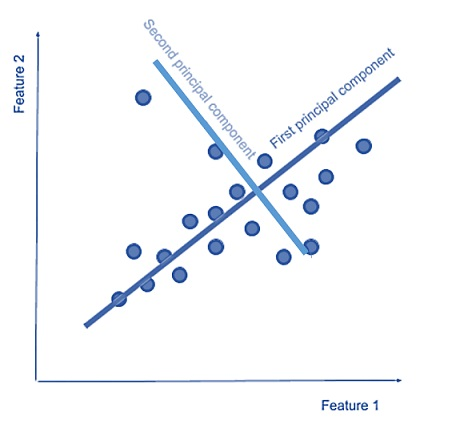
\includegraphics[width=6.44in]{img/w10-PCA} 

}

\caption{Figure 1. Illustration of PCA. The least (2nd) important component can be used for anomaly detection.}\label{fig:unnamed-chunk-1}
\end{figure}

\hypertarget{linear-discriminant-analysis-lda}{%
\subsection{Linear Discriminant Analysis
(LDA)}\label{linear-discriminant-analysis-lda}}

Linear discriminant analysis (LDA) also creates linear combinations of
your original features. However, unlike PCA, LDA doesn't maximize
explained variance. Instead, it maximizes the separability between
classes.

In other words, the goal of an LDA is to project a feature space (a data
set n-dimensional samples) onto a smaller subspace k (where
\(k \le n−1\)) while maintaining the class-discriminatory information.

In general, dimensionality reduction does not only help reduce
computational costs for a given classification task, but it can also be
helpful to avoid overfitting by minimizing the error in parameter
estimation (``curse of dimensionality'').

\begin{figure}

{\centering 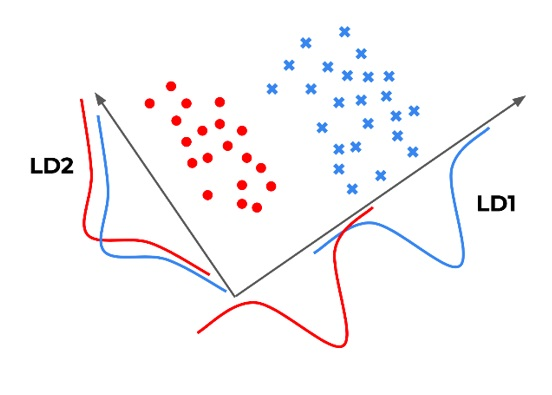
\includegraphics[width=7.67in]{img/w10-LDA} 

}

\caption{Figure 2. Illustration of LDA.}\label{fig:unnamed-chunk-2}
\end{figure}

Therefore, LDA is a supervised method that can only be used with labeled
data. The LDA transformation is also dependent on scale, so we should
normalize original features in the data set first.

\textbf{Strengths}: LDA is supervised, which can (but doesn't always)
improve the predictive performance of the extracted features.
Furthermore, LDA offers variations (i.e.~quadratic LDA) to tackle
specific roadblocks.

\textbf{Weaknesses}: As with PCA, the new features are not easily
interpretable, and we must still manually set or tune the number of
components to keep. LDA also requires labeled data.

\textbf{PCA vs LDA}: Which is better? The results will vary from problem
to problem. In other words, the \textbf{No Free Lunch} Theorem applies
to this situation. The following figure depicts the difference between
PCA and LDA.

\begin{figure}

{\centering 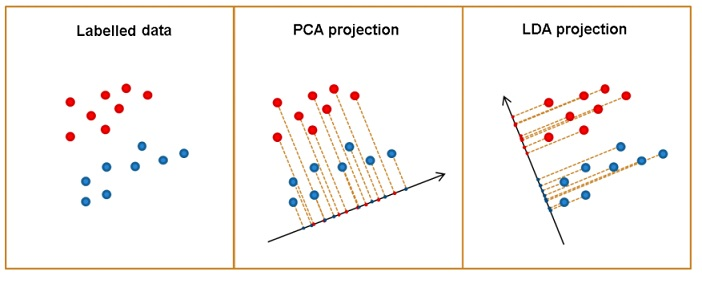
\includegraphics[width=9.75in]{img/w10-LDA-vs-LDA} 

}

\caption{Figure 3. Illustration of the difference of PCA and LDA.}\label{fig:unnamed-chunk-3}
\end{figure}

\hypertarget{case-study-lda-with-iris-data}{%
\subsection{Case-study: LDA with Iris
Data}\label{case-study-lda-with-iris-data}}

like PCA whose mathematical formulation involves matrix algebra
(eigenvector and eigenvalues) and linear programming (optimization with
linear constraints), in LDA we still need to use the same tools but with
different objective functions for optimization. We will not introduce
these mathematical steps to find the linear discriminant components.

Next, we use R function \textbf{lda()} in library \textbf{\{MASS\}} to
find LDA components based on the four numerical features in Iris data.

\textbf{lda()} returns several results:

\begin{itemize}
\item
  The most important result here is the coefficients, they are values
  that describe the new feature space where the data will be projected
  in.
\item
  LDA reduces dimensionality from the original number of features to C
  --- 1 features, where C is the number of classes. In this case, we
  have 3 classes, therefore the new feature space will have only 2
  features.
\end{itemize}

\begin{Shaded}
\begin{Highlighting}[]
\FunctionTok{data}\NormalTok{(iris)}
\CommentTok{\# Data partition}
\NormalTok{training\_sample }\OtherTok{\textless{}{-}} \FunctionTok{sample}\NormalTok{(}\FunctionTok{c}\NormalTok{(}\ConstantTok{TRUE}\NormalTok{, }\ConstantTok{FALSE}\NormalTok{), }\FunctionTok{nrow}\NormalTok{(iris), }\AttributeTok{replace =}\NormalTok{ T, }\AttributeTok{prob =} \FunctionTok{c}\NormalTok{(}\FloatTok{0.6}\NormalTok{,}\FloatTok{0.4}\NormalTok{))}
\NormalTok{train }\OtherTok{\textless{}{-}}\NormalTok{ iris[training\_sample, ]}
\NormalTok{test }\OtherTok{\textless{}{-}}\NormalTok{ iris[}\SpecialCharTok{!}\NormalTok{training\_sample, ]}
\CommentTok{\#}
\NormalTok{lda.iris }\OtherTok{\textless{}{-}} \FunctionTok{lda}\NormalTok{(Species }\SpecialCharTok{\textasciitilde{}}\NormalTok{ ., }\AttributeTok{data =}\NormalTok{ train)}\CommentTok{\#, prior = rep(1/3, 3))}
\FunctionTok{kable}\NormalTok{(lda.iris}\SpecialCharTok{$}\NormalTok{scaling, }\AttributeTok{caption=}\StringTok{"The scaling coefficients of LDA"}\NormalTok{)  }\CommentTok{\# show results}
\end{Highlighting}
\end{Shaded}

\begin{longtable}[]{@{}lrr@{}}
\caption{The scaling coefficients of LDA}\tabularnewline
\toprule\noalign{}
& LD1 & LD2 \\
\midrule\noalign{}
\endfirsthead
\toprule\noalign{}
& LD1 & LD2 \\
\midrule\noalign{}
\endhead
\bottomrule\noalign{}
\endlastfoot
Sepal.Length & 0.5109187 & -0.5246074 \\
Sepal.Width & 1.6950374 & -1.8070226 \\
Petal.Length & -1.8050731 & 1.2966957 \\
Petal.Width & -3.4669482 & -3.1194567 \\
\end{longtable}

The two new feature variables based on the two LDA are explicitly given
by

\[
LDA_1 = (0.51\times Sepal.Length) + (1.96\times Sepal.Width) + (-2.12\times Petal.Length) + (-2.98\times Petal.Width) 
\] \[
LDA_2 = (-0.76\times Sepal.Length) + (2.85\times Sepal.Width) + (-1.05\times Petal.Length) + (1.92\times Petal.Width)
\] Next, we use LDA to make a prediction using the hold-out test data.
Note that predict() returns three objects with three different pieces of
information:

\begin{itemize}
\tightlist
\item
  \textbf{lda.test\$class} contains the predicted labels.
\item
  \textbf{lda.test\$posterior} contains the predictive class
  probabilities of new data points.
\item
  \textbf{lda.test\$x} contains the two LDA scores.
\end{itemize}

In the following code, we extract the predicted labels and then compare
them with the actual labels to find the confusion matrix and calculate
the accuracy of classification LDA.

\begin{Shaded}
\begin{Highlighting}[]
\NormalTok{lda.test }\OtherTok{\textless{}{-}} \FunctionTok{predict}\NormalTok{(lda.iris, }\AttributeTok{newdata =}\NormalTok{ test)}
\NormalTok{test}\SpecialCharTok{$}\NormalTok{lda }\OtherTok{\textless{}{-}}\NormalTok{ lda.test}\SpecialCharTok{$}\NormalTok{class  }
\NormalTok{confusion.matrix }\OtherTok{=} \FunctionTok{table}\NormalTok{(test}\SpecialCharTok{$}\NormalTok{lda,test}\SpecialCharTok{$}\NormalTok{Species)}
\FunctionTok{kable}\NormalTok{(confusion.matrix, }\AttributeTok{caption =} \StringTok{"Confusion matrix based one LDA."}\NormalTok{)}
\end{Highlighting}
\end{Shaded}

\begin{longtable}[]{@{}lrrr@{}}
\caption{Confusion matrix based one LDA.}\tabularnewline
\toprule\noalign{}
& setosa & versicolor & virginica \\
\midrule\noalign{}
\endfirsthead
\toprule\noalign{}
& setosa & versicolor & virginica \\
\midrule\noalign{}
\endhead
\bottomrule\noalign{}
\endlastfoot
setosa & 21 & 0 & 0 \\
versicolor & 0 & 22 & 0 \\
virginica & 0 & 1 & 21 \\
\end{longtable}

The accuracy of LDA prediction on the test data set is \(49/50 = 98\%\).

\hypertarget{remarks}{%
\subsection{Remarks}\label{remarks}}

We have introduced two well-known feature extraction methods: PCA and
LDA. Both are linear extraction methods. PCA is an unsupervised
extraction method and LDA is a supervised method. Both methods are
developed for different purposes but both can be used for dimensional
reduction.

Both PCA and LDA can be adapted for nonlinear feature extraction by
introducing kernel functions (i.e., kernel PCA and kernel LDA) or
changing the linear combination of the original features into the
polynomial expression to capture the nonlinear patterns (i.e.,
polynomial PCA and polynomial LDA).

The various variable transformations including the well-known Box-Cox
transformation, discretization, and redefining categorical variables by
combing categories in meaningful ways are all called feature extraction
methods.

\hypertarget{feature-extraction-with-serial-data}{%
\section{Feature Extraction with Serial
Data}\label{feature-extraction-with-serial-data}}

The feature extraction methods introduced in the previous section are
based on cross-sectional data. There are only very limited discussions
on feature extraction based on serial data including time series and
panel data. In particular, no feature extraction method based on panel
data has been discussed so far in the literature.

In this section, we first introduce the way and type of features one can
extract from a time series. Then we introduce a new method for
extracting features from panel data. This method can also be used to
define a feature based on the regular time series. The new method
borrows the idea of the formulation of the process capability index in
statistical process and quality control.

\hypertarget{feature-extraction-with-time-series}{%
\subsection{Feature Extraction with Time
Series}\label{feature-extraction-with-time-series}}

Time series data is data that is collected at different points in time.
This is opposed to cross-sectional data which observes individuals,
companies, etc. at a single point in time.

Because data points in time series are collected at adjacent time
periods there is potential for correlation between observations. This is
one of the features that distinguishes time-series data from
cross-sectional data.

Time series data can be found in economics, social sciences, finance,
epidemiology, and the physical sciences.

\begin{figure}

{\centering 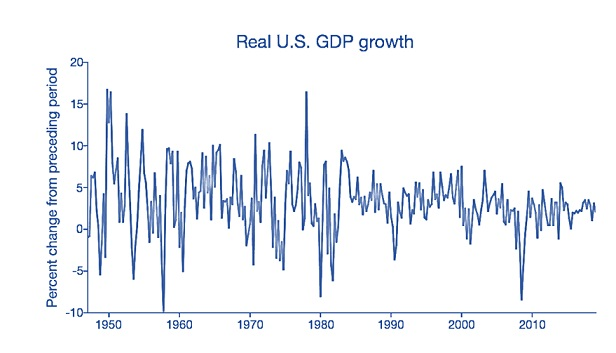
\includegraphics[width=8.56in]{img/w10-What-is-TS} 

}

\caption{Figure 4. Illustration of times patterns.}\label{fig:unnamed-chunk-6}
\end{figure}

There are two main goals of time series analysis: identifying the nature
of the phenomenon represented by the sequence of observations, and
forecasting (predicting future values of the time series variable).

\hypertarget{statistical-models}{%
\subsubsection{Statistical Models}\label{statistical-models}}

The most common and effective statistical methods of Forecasting are
Simple Moving Average (SMA), Exponential Smoothing (SES),
Auto-regressive Integration Moving Average (ARIMA).

We will not discuss these methods in this note but will introduce the
exponential smoothing method for the time series next week.

\hypertarget{machine-learning-algorithms}{%
\subsubsection{Machine Learning
Algorithms}\label{machine-learning-algorithms}}

One of the most important properties an algorithm needs in order to be
considered a time-series algorithm is the ability to extrapolate
patterns outside of the domain of training data. Many machine learning
algorithms do not have this capability, as they tend to be restricted to
a domain that is defined by training data. Therefore, they are not
suited for time series, as the objective of time series is to project
into the future.

Another important property of a time series algorithm is the ability to
derive confidence intervals. While this is a default property of time
series models, most machine learning models do not have this ability
because they are not all based on statistical distributions.

There are also machine learning models such as neural network models
that can be applied to time series which use \texttt{lagged\ predictors}
and can handle \texttt{extracted\ features}, such as Neural Networks
Autoregression (NNAR). There are even time-series models borrowed from
deep learning, specifically in the RNN (Recurrent Neural Network)
family. The following figure shows how to use extracted features in a
neural network model for forecasting.

\begin{figure}

{\centering 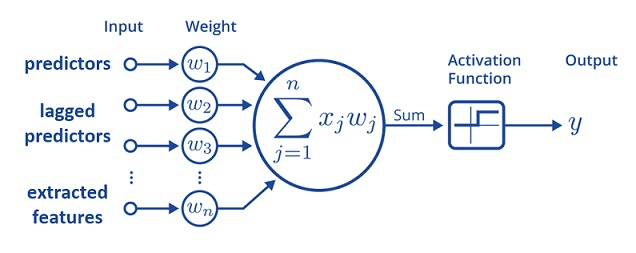
\includegraphics[width=8.83in]{img/w10-ANN-TS} 

}

\caption{Figure 5. How to ANN to model time series.}\label{fig:unnamed-chunk-7}
\end{figure}

\hypertarget{feature-extraction-for-time-series}{%
\subsubsection{Feature Extraction for Time
Series}\label{feature-extraction-for-time-series}}

Since the machine learning method can incorporate both lagged predictors
and additional features to improve the forecast accuracy, we can extract
some features from the underlying features. The following figure
illustrates the process of how to extract features from time-series
data.

\begin{figure}

{\centering 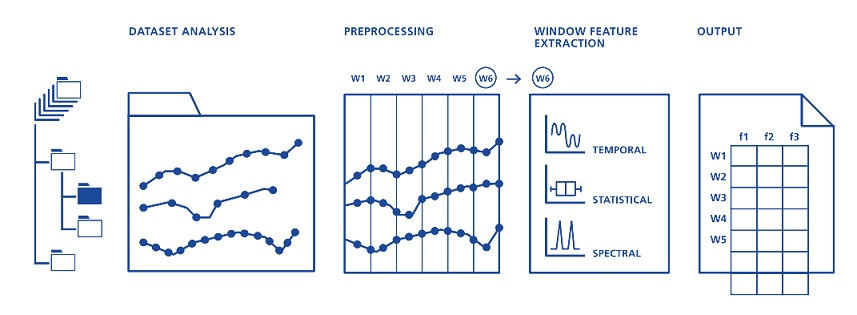
\includegraphics[width=11.9in]{img/w10-Serial-Feature-Extraction} 

}

\caption{Figure 6. How to extract features from time series.}\label{fig:unnamed-chunk-8}
\end{figure}

As shown in the above figure, three types of features can be extracted
from time-series data.

\begin{itemize}
\item
  \textbf{Temporal features (time-domain features)} are simple to
  extract and have an easy physical interpretation.
\item
  \textbf{Statistical features} are mainly descriptive statistics such
  as windowed mean, median, skewness, etc.
\item
  \textbf{Spectral features (frequency-based features)} are obtained by
  converting the time-based signal into the frequency domain.
\end{itemize}

These features are descriptive and can be easily automated. Some
software programs have been made to extract these types of features
automatically in practice.

\hypertarget{model-based-feature-extraction-with-panel-data}{%
\subsection{Model-based Feature Extraction with Panel
Data}\label{model-based-feature-extraction-with-panel-data}}

This subsection focuses on a new feature extraction method that extracts
information based on models and algorithms from sequential data. The
algorithm borrows the idea of measuring the process information (such as
capability and quality) through the sequence data generated by the
process.

Since this is a model-based algorithm, it is more powerful than those
features extracted from the time series discussed in the previous
subsection.

\hypertarget{concepts-process-capability-and-control-chart}{%
\subsubsection{Concepts Process Capability and Control
Chart}\label{concepts-process-capability-and-control-chart}}

Process control is the ability to monitor and adjust a process to give
the desired output. It is used in the industry to maintain quality and
improve performance. Key tools in process control include control chart,
process capability index, etc.

Both control chart and process capability index use the same key
characteristics of the underlying process in their construction:

\begin{itemize}
\item
  \textbf{Specification limits} can be defined as targets that are set
  for a particular process or a product either by the customer or based
  on the performance of the market. In other words, it can also be
  defined as a result that is expected from a particular metric.
  Specification limits are set by customers or the management.
\item
  \textbf{Control limits} on the other hand help in indicating the
  changes which occur in the performance of a particular process.
  Control limits also provide real-time value. Control limits are
  dependent on the underlying process.
\end{itemize}

Control limits can be either upper control limit (UCL) or lower control
limit (LCL). Similarly, specification limits can be either upper
specification limit (USL) or lower specification limit (LSL).

\begin{figure}

{\centering 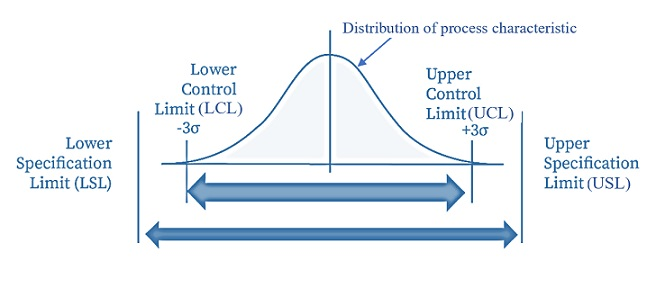
\includegraphics[width=9.11in]{img/w10-control-spec-limits} 

}

\caption{Figure 7. Structure of a control chart.}\label{fig:unnamed-chunk-9}
\end{figure}

\textbf{Understanding the control chart}

Several concepts will be used in the definition of the process
capability index.

Control charts are one of the most popular SPC tools used by
manufacturers. They are used to determine \textbf{whether a process is
in- or out-of-control}.

When points on a control chart move outside the upper or lower control
limit, the process are said to be \textbf{``out-of-control.''} As long
as the points are within control limits, the process is
\textbf{``in-control''}. An \textbf{out-of-control process} could
produce defective parts. However, if a point is outside the
\textbf{specification limits}, the process produces defective products.

\begin{figure}

{\centering 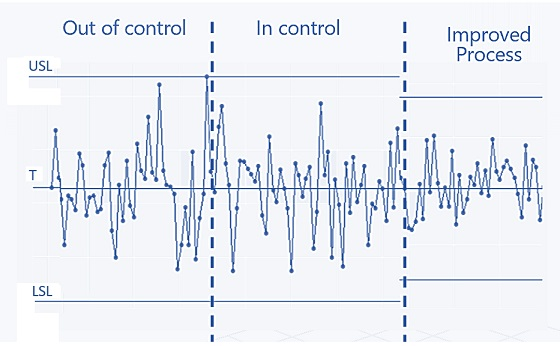
\includegraphics[width=7.78in]{img/w10-control-chart} 

}

\caption{Figure 8. In-control and out-of-control processes.}\label{fig:unnamed-chunk-10}
\end{figure}

Control charts are visual tools for monitoring the process capability.
With a control chart, we can see the potential shift of process mean and
variation at the same time. A numerical measure that can be defined to
capture both aforementioned shifts of a process in a single number is
the process capability index (PCI).

\hypertarget{concept-of-process-capability-index-pci}{%
\subsubsection{Concept of Process Capability Index
(PCI)}\label{concept-of-process-capability-index-pci}}

Process capability index measures the degree of variation an in-control
process experiences relative to its specification limits. It can also be
used to compare different processes with respect to the optimal
situation or if they come up to our expectations.

The first process capability index is defined by \(C_p\),

\[
C_p = \frac{USL-LSL}{6\sigma}
\]

which is an estimate of what the process is capable of producing if the
process mean were to be centered between the specification limits,
assuming that the process output is approximately normally distributed.
This first \(C_p\) was invented and used in the Japanese semiconductor
industry in the 1970s.

\begin{figure}

{\centering 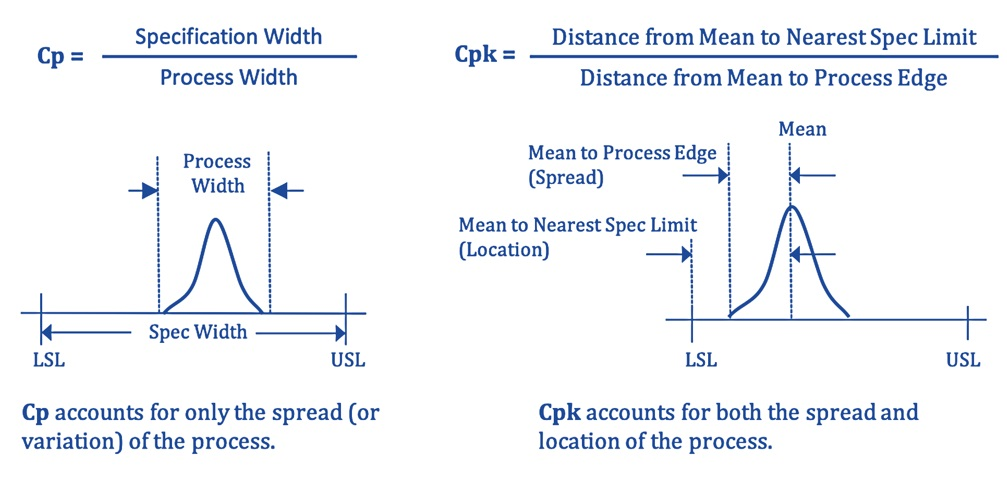
\includegraphics[width=13.99in]{img/w10-1st-2nd-generation-PCIs} 

}

\caption{Figure 9. First and second generation PCIs.}\label{fig:unnamed-chunk-11}
\end{figure}

Since \(C_p\) does not consider process means and process target,
several major families of PCIs were defined after \(C_p\). The following
table lists major PCIs used in the industry for various purposes.

\begin{center}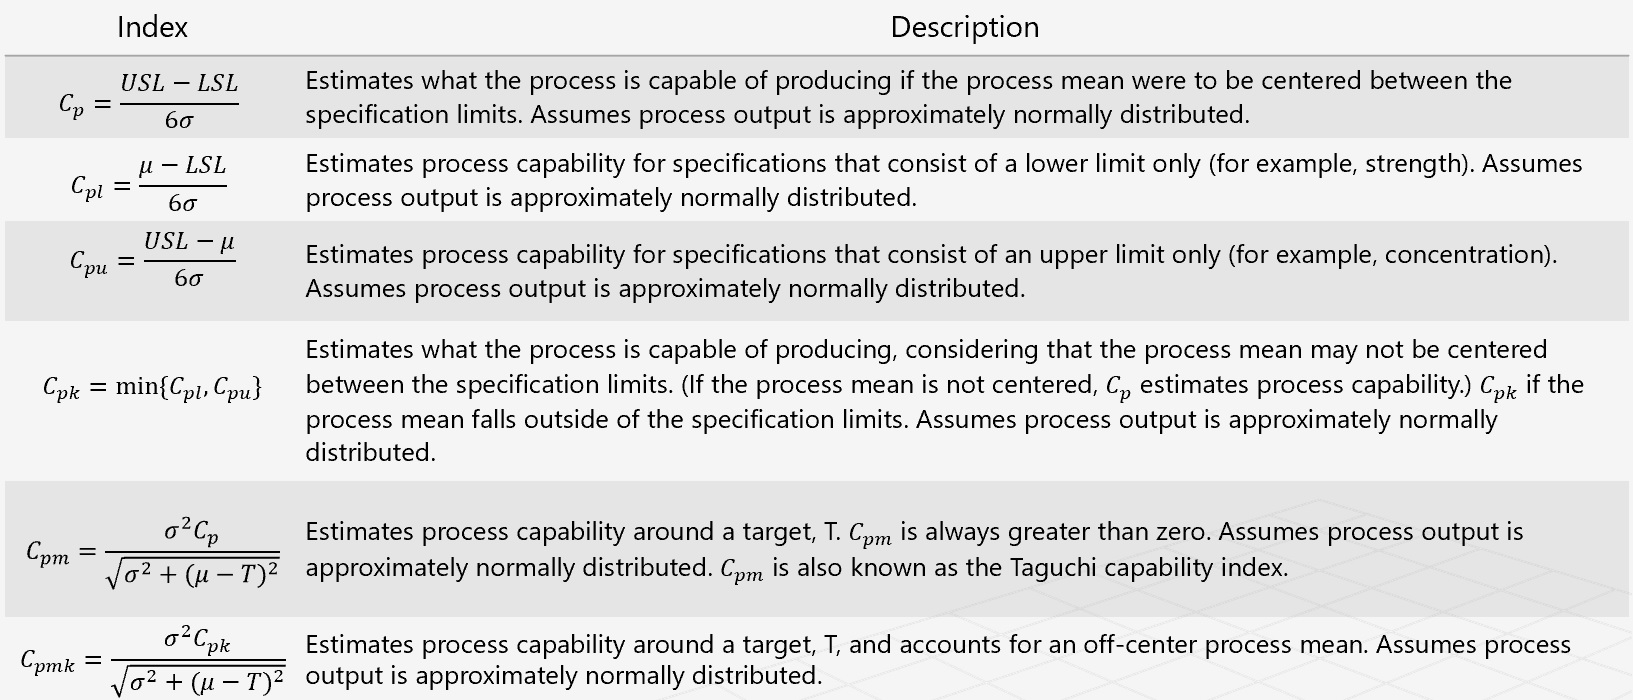
\includegraphics[width=22.68in]{img/w10-list-of-PCIs} \end{center}

In the manufacturing industry, PCIs are used to measure the quality of a
process (product), USL, and LSL and T (target) are given by customers or
the management. When applying PCI in other fields such as fraud
detection, USL, LSL and T are not given, we need to figure out a way to
obtain reasonable USL, LSL, and T in order to define the PCI. The next
subsection explains the idea of using PCI to define fraud index.

\hypertarget{framework-of-fraud-index-based-on-pci}{%
\subsubsection{Framework of Fraud Index Based on
PCI}\label{framework-of-fraud-index-based-on-pci}}

We can consider a credit card as \textbf{a process} that produces
transactions. This process characterizes the card holder's spending
behavior. For an established credit card account, we can segment the
spending in different subcategories and define different sub-processes.
A PCI can be defined for each sub-process. The question is that there
are no specification limits set to these types of ``processes''. We need
to use historical data to obtain optimal specification limits in order
to define quality PCIs.

The following chart explains the idea of how to define PCI for a process
without being given pre-set process limits.

\begin{figure}

{\centering 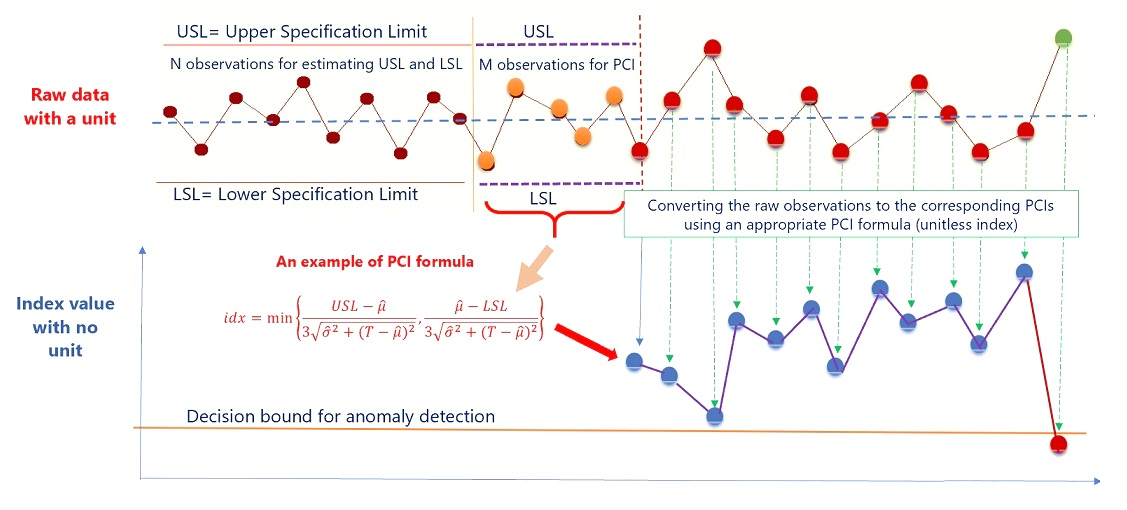
\includegraphics[width=15.65in]{img/w10-Rolling-PCIs} 

}

\caption{Figure 10. Illustration of defining PCI of a process without given process limits}\label{fig:unnamed-chunk-13}
\end{figure}

Since fraud detection is a real-time process, the fraud index must also
be defined in real-time. The above explains how real-time PCI can be
defined. The PCI defined in the above illustration is a rolling PCI
since its specification limits are changing over time. The specification
limits can also be set as hyperparameters. We can then search for
optimal hyperparameters to define optimal PCI for fraud detection.

\end{document}
